
\documentclass[12pt]{article}
\usepackage{amsmath, amssymb}
\usepackage{geometry}
\usepackage{graphicx}
\usepackage{hyperref}
\geometry{margin=1in}

\title{A Cyclic 4D-Time Universe Model: Bounce, Expansion, and Turnaround Controlled by Closed Time Geometry}
\author{Your Name}
\date{\today}

\begin{document}
\maketitle

\begin{abstract}
We propose a toy cosmological framework in which the fourth dimension (time) is not infinite,
but cyclic and bounded. This closed time geometry forces both the initiation of cosmic expansion
(the bounce) and its termination (the turnaround), eliminating the need for external triggers.
We sketch an effective Friedmann equation with Loop Quantum Cosmology--inspired quantum corrections
to avoid singularities and show how a large-$a$ turnaround can be incorporated via curvature or an
effective negative cosmological term. The bounce is interpreted as a single-frame quantum state,
linking emergent spacetime ideas to cyclic cosmology.
\end{abstract}

\section{Introduction}
We outline the singularity problem in general relativity, the entropy challenge in cyclic models,
and why a closed time geometry naturally sets the endpoints of expansion without ad hoc switches.

\section{Framework}
\subsection{Cyclic Time Ansatz}
Define periodic cosmic time $\tau\in[0,T)$ with $a(\tau+T)=a(\tau)$, and boundary conditions
\begin{equation}
a(0)=a_{\min}>0,\quad \dot a(0)=0,\qquad a(T/2)=a_{\max},\quad \dot a(T/2)=0.
\end{equation}

\subsection{Effective Friedmann Equation}
Inspired by Loop Quantum Cosmology, use
\begin{equation}
H^2=\left(\frac{\dot a}{a}\right)^2=\frac{8\pi G}{3}\,\rho(a)\left(1-\frac{\rho(a)}{\rho_c}\right)
+\frac{\Lambda}{3}-\frac{k}{a^2},
\end{equation}
with $\rho(a)=\rho_{r0}a^{-4}+\rho_{m0}a^{-3}+\rho_\Lambda$ (toy) and critical density $\rho_c$.
The $(1-\rho/\rho_c)$ factor generates a bounce at small $a$; $\Lambda<0$ or $k>0$ yields a
large-$a$ turnaround.

\section{Results (Toy Examples)}
\subsection{Cyclic Scale Factor}
Figure~\ref{fig:atau} shows a periodic $a(\tau)$ with bounce and turnaround (toy ansatz).

\begin{figure}[h]
\centering
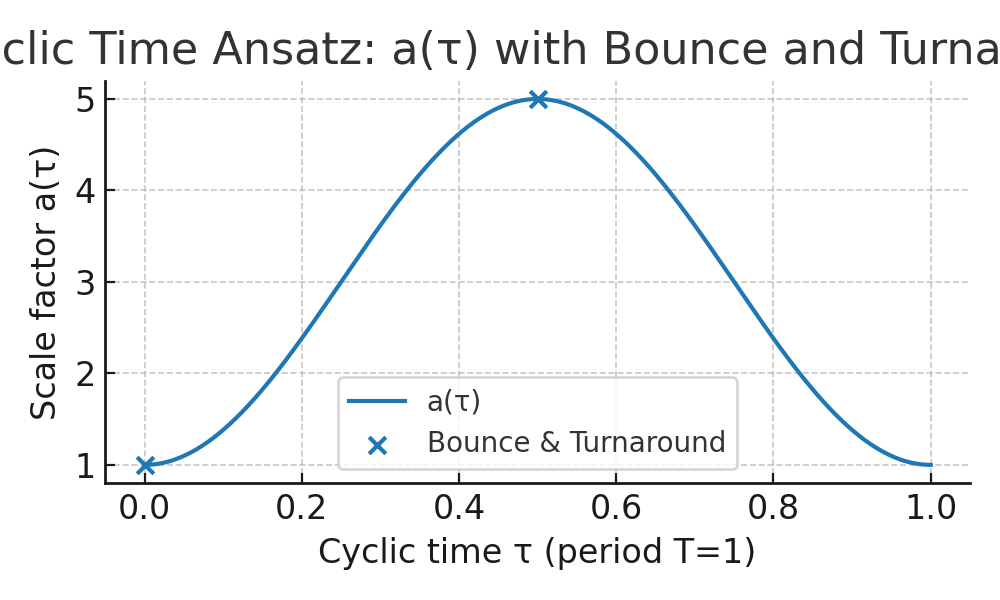
\includegraphics[width=0.7\linewidth]{figures/plot_a_tau.png}
\caption{Cyclic time ansatz: $a(\tau)$ with bounce ($\tau=0$) and turnaround ($\tau=T/2$).}
\label{fig:atau}
\end{figure}

\subsection{Effective $H^2(a)$ with Two Turning Points}
Figure~\ref{fig:h2a} shows a toy effective $H^2(a)$ with a bounce at small $a$ and a turnaround at large $a$.

\begin{figure}[h]
\centering
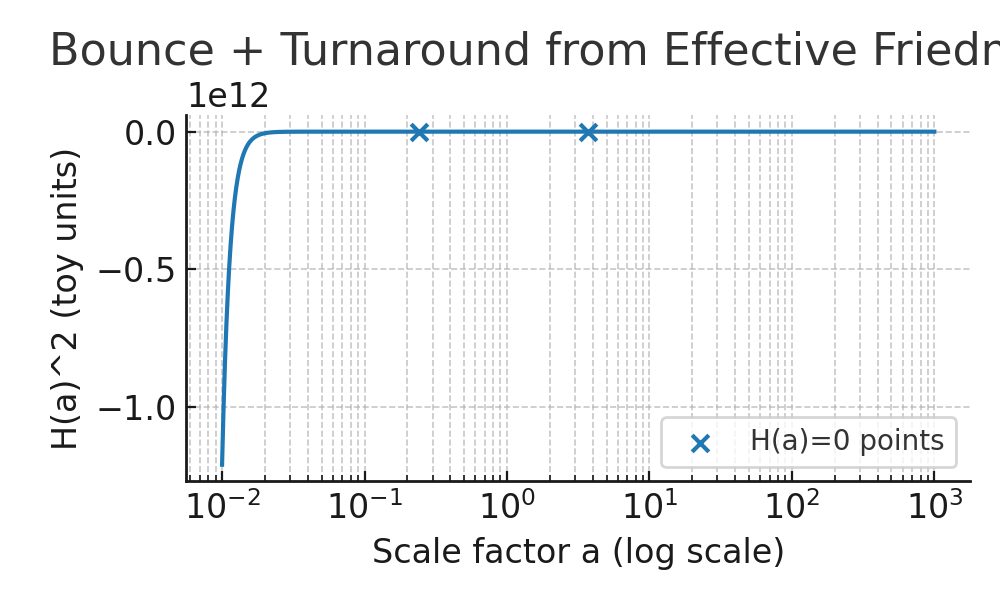
\includegraphics[width=0.7\linewidth]{figures/plot_H2.png}
\caption{Toy $H^2(a)$ exhibiting a small-$a$ bounce and a large-$a$ turnaround.}
\label{fig:h2a}
\end{figure}

\section{Discussion}
We compare the cyclic 4D-time controller with Loop Quantum Cosmology bounces, cyclic/ekpyrotic models,
and Conformal Cyclic Cosmology, highlighting how a closed time geometry can address both the singularity
and ``end of expansion'' problems in one stroke.

\section{Conclusions and Next Steps}
We sketched a minimal, self-consistent toy model embodying the idea of time as a closed controller loop.
Future work: derive the effective dynamics from a deeper theory, propose observational discriminants,
and analyze entropy flow across cycles.

\section*{Acknowledgments}
(Place acknowledgments here.)

\section*{References}
(Add detailed references here.)

\end{document}
